\chapter{Risposte orale Paganelli}
\section{Hidden terminal}

\begin{figure}[htbp]
   \centering
   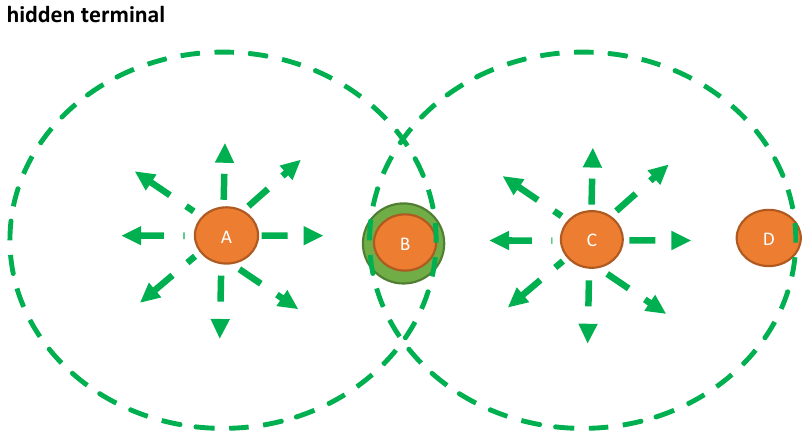
\includegraphics{images/questions/Schermata del 2023-11-01 15-19-50.png}
   % \caption{}
   \label{fig:dom2.1}
\end{figure}

Una delle sfide dei terminali nelle reti wireless è la limitata conoscenza dei terminali che non sono nel loro raggio d'azione. \\
Il problema degli hidden terminal è un problema che si verifica quando due o più station che sono rispettivamente fuori dal range dell'altra vogliono trasmettere in modo simultaneo allo stesso device, generando in questo modo delle collisioni.

Nell'immagine è possibile osservare come il nodo A risulti essere un hidden terminal per il nodo C e viceversa durante le rispettive comunicazioni con B. Questo accade perché A, non essendo nel radio range di C, non sarebbe in grado di rilevare un'eventuale comunicazione da C verso B. Quindi, se A iniziasse a comunicare con B mentre C sta già comunicando con B, questo porterebbe ad una collisione in B.

\section{Exposed terminal}

\begin{figure}[htbp]
   \centering
   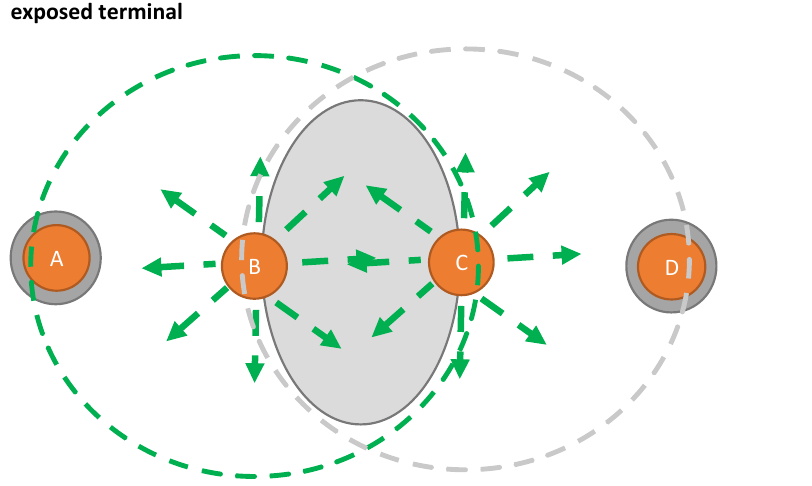
\includegraphics{images/questions/Schermata del 2023-11-01 15-26-25.png}
   % \caption{}
   \label{fig:dom2.2}
\end{figure}

Il problema degli exposed terminal è un problema che si verifica quando una stazione è esposta alle comunicazioni di un'altra stazione e risulta essere impossibilitata ad inviare messaggi a sua volta, anche quando le comunicazioni non sono rivolte verso lo stesso terminale.

Nell'immagine è possibile osservare come il nodo C sia esposto alla comunicazione da B verso A, impedendo una possibile comunicazione da C verso D, che potrebbe comunque avvenire in parallelo.

\section{RTS/CTS}

\begin{figure}[htbp]
   \centering
   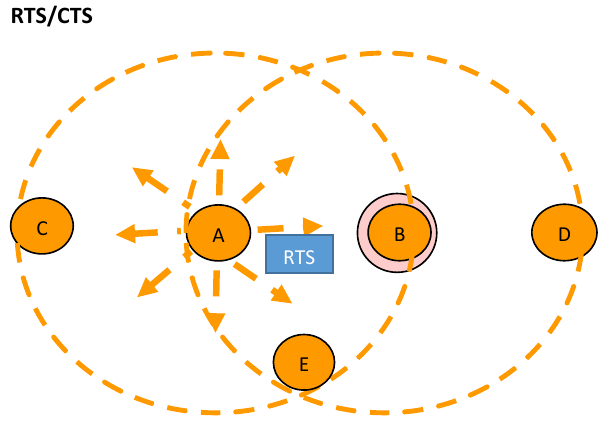
\includegraphics{images/questions/Schermata del 2023-11-01 15-42-48.png}
   % \caption{}
   \label{fig:dom2.3}
\end{figure}

Il meccanismo dei RTS (Request To Send) e dei CTS (Clear To Send) viene utilizzato all'interno del protocollo MACA (Multiple Access with Collision Avoidance). In questo protocollo, per cercare di evitare (non risolvere) le collisioni e il problema degli hidden/exposed terminal viene inviato uno short frame precedentemente all'invio del data frame, così da far astenere gli altri dispositivi dall'invio di messaggi.

Nell'immagine è mostrata la comunicazione dal nodo A al nodo B:
\begin{itemize}
    \item Il nodo A invia un RTS (Request-to-send) al nodo B, che viene ricevuto anche dai nodi C e da E. L'RTS contiene anche la lunghezza del data frame.
    \item Successivamente B, pronto ad accettare il messaggio, risponde ad A con un CTS (Clear-to-send), che viene ricevuto dai nodi A, D ed E.
    \item A questo punto, A può inviare il data frame a B.
\end{itemize}
Questo protocollo però non risolve il problema degli hidden/exposed terminal. Infatti, C è un exposed terminal, in quanto riceve l'RTS di A ma non il CTS di B: quindi C è libero di trasmettere, ma tutto quello che riceverà farà collisione con i dati mandati da A; D è un hidden terminal perché riceve il CTS da B ma non l'RTS da A, quindi D non può più trasmettere fino a quando la trasmissione del data frame è completata \textred{Trasmissione che non sentirà. MACAW aggiunge un ACK finale ---a ricezione dati ultimata--- inviato da B per ovviare al problema, (giusto?)}.

Cosa accade se B e C mandano contemporaneamente l'RTS al nodo A? C'è collisione tra gli RTS, quindi non viene generato un CTS. La soluzione al problema consiste nell'utilizzo da parte di B e C del \textit{Binary Exponential Backoff} per provare a rinviare l'RTS.

Cosa accade se un nodo al di fuori del range di A e B prova a comunicare con E? E non risponderà all'RTS del nodo esterno, dato che E ha sentito il CTS di B. Il nodo esterno proverà (sempre utilizzando \textit{Binary Exponential Backoff}) a rinviare l'RTS fino a quando E non risponderà.

\note{MACAW (MACA for Wireless networks) è un miglioramento del protocollo MACA: aggiunge ACK frame inviato dal nodo ricevente per fare l'acknowledge dei dati ricevuti, e altri meccanismi per scambio di informazioni: il Data Sending frame, inviato dal mittente quando inizia a inviare informazioni; il RRTS (Request to RTS), inviato da un nodo che ha ricevuto un RTS, ma non era in grado di rispondere a causa di un'altra comunicazione attiva.}

\section{MN indirect routing}

\begin{figure}[htbp]
   \centering
   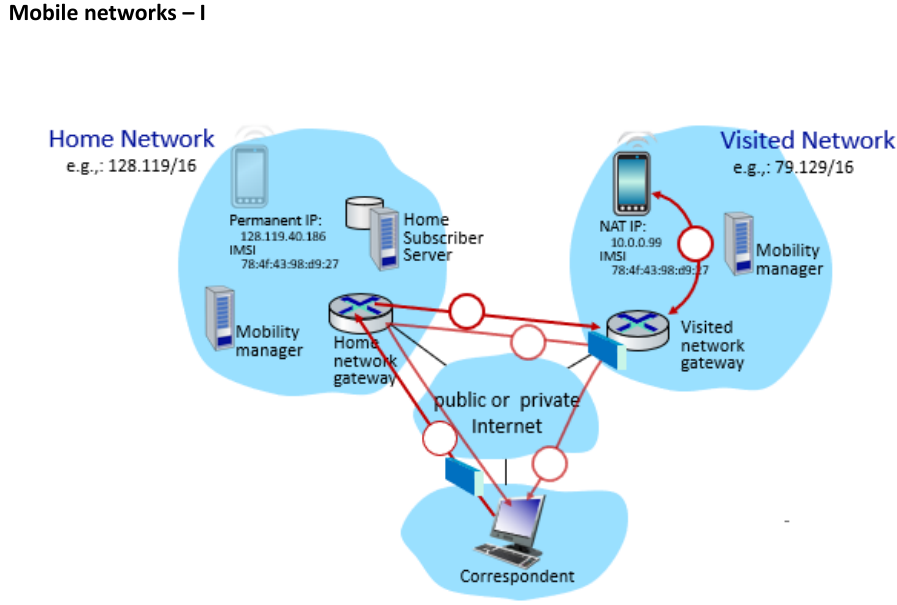
\includegraphics{images/questions/Schermata del 2023-11-01 16-14-28.png}
   % \caption{}
   \label{fig:dom2.4}
\end{figure}

L'immagine mostra il funzionamento dell'\textbf{\emph{indirect routing}} per la mobilità tra una home network e una visited network. La home network rappresenta la rete ``nativa'' di un dispositivo con un abbonamento ad un mobile provider (e.g. \textit{Verizon}), dove le informazioni relative ai device abbonati vengono salvate nel HHS (Home Subscriber Server). Il visited network è un qualsiasi altro network gestito da un provider diverso da quello con cui il device è abbonato.

Nell'indirect routing sono necessari tre protocolli fondamentali:
\begin{itemize}
\item un protocollo di associazione mobile-device-to-visited-network, che permette l'associazione alla visited network quando si entra in contatto con questa e viceversa la disassociazione quando il dispositivo lascia la visited network;
\item un protocollo di registrazione visited-network-to-home-network-HSS, che permette alla visited network di registrare la posizione del device mobile dentro l'HSS della sua home network.
\item un protocollo di datagram tunneling tra home network gateway e il visited network gateway routers, necessario per effettuare incapsulamento e forwarding, da parte dell'home network gateway verso la visited network gateway, e decapsulamento, traduzione NAT e forwarding  da parte del visited network gateway verso il mobile device.
\end{itemize}

Vediamo i passi descritti nella figura:
\begin{enumerate}
    \item Il mittente (Correspondent) utilizza l'home address del device con cui vuole comunicare come indirizzo di destinazione del datagram.
    \item Il home network gateway riceve il datagram, e lo inoltra (utilizzando il precedentemente descritto protocollo di \textit{tunneling}) al visited network gateway, dopo aver consultato il HSS per scoprire la posizione del dispositivo mobile.
    \item Il visited network gateway inoltra il datagramma al dispositivo mobile (tipicamente dopo aver utilizzato NAT) 
    \item Il visited gateway router inoltra la risposta al mittente (Correspondant) direttamente (\textbf{b}) o utilizzando la home network (\textbf{a}).
\end{enumerate}

\note{L'indirect routing risulta inefficiente nel caso in cui un dispositivo B è un dispositivo mobile che si è spostato dalla sua home network alla stessa rete del dispositivo A (mittente, che in questo caso ha home network diversa). Nonostante entrambi i dispositivi si trovino ora nella stessa rete, l'instradamento dei messaggi dal Dispositivo A al Dispositivo B non avviene direttamente. Invece, segue questo il percorso a 'triangolo' dell'indirect routing, portando ad un overhead non necessario.}

\note{Il IMSI (o International Mobile Subscriber Identifier) viene utilizzato come una sorta di MAC address del device per poterlo identificare, insieme al suo Permanent IP assegnato dal suo home network. Per far riferimento a un mobile device durante l'invio dei messaggi, viene utilizzato il suo IP permanente come riferimento; Per far riferimento a un mobile device per billing, autenticazione, ecc.., viene utilizzato il suo IMSI come riferimento.}

\section{MN direct routing}

\begin{figure}[htbp]
   \centering
   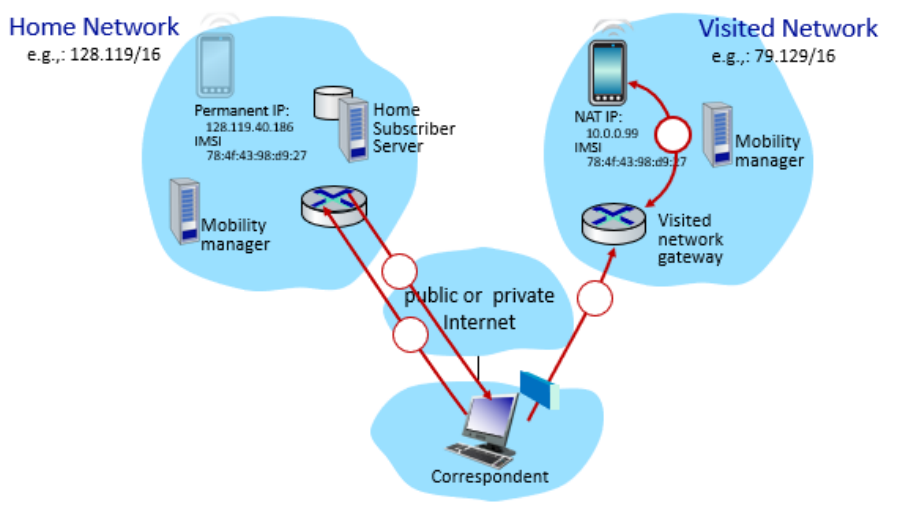
\includegraphics{images/questions/Schermata del 2023-11-02 10-20-15.png}
   % \caption{}
   \label{fig:dom2.5}
\end{figure}

L'immagine mostra il funzionamento del \textbf{\emph{direct routing}} per la mobilità tra una home network e una visited network. La home network rappresenta la rete "nativa" di un dispositivo con un abbonamento ad un mobile provider (e.g. \textit{Verizon}), dove le informazioni relative ai device abbonati vengono salvate nel HHS (Home Subscriber Server). Il visited network è un qualsiasi altro network gestito da un provider diverso da quello con cui il device è abbonato.

A differenza dell'indirect routing, in cui le comunicazioni tra Correspondent e dispositivo mobile passano dalla home network, utilizzando il direct routing il mittente (Correspondent) invia direttamente il datagram packet al dispositivo mobile nella visited network:
\begin{enumerate}
    \item Il mittente (Correspondent) contatta la home network del dispositivo mobile a cui vuole mandare un messaggio attraverso il suo indirizzo IP permanente.
    \item La home network risponde al mittente (dopo aver chiesto al HSS) con l'IP assegnato al dispositivo mobile nella visited network.
    \item Il mittente (Correspondent) invia il messaggio al mobile device utilizzando l'IP appena ottenuto.
    \item Il visited network gateway inoltra il datagramma al dispositivo mobile (tipicamente dopo aver utilizzato NAT)
\end{enumerate}

\note{Il direct routing risolve il problema del 'triangle routing', a costo però di non essere trasparente nei confronti del Correspondent, visto che deve procurarsi da solo l'indirizzo assegnato al mobile device dalla visited network. Nell'indirect routing il Correspondent non deve gestire la mobilità del dispositivo mobile (che può anche avvenire più volte in un breve periodo), rendendo l'indirect routing il protocollo più utilizzato.}

\section{MN HO tra BS nella stessa rete}

\begin{figure}[htbp]
   \centering
   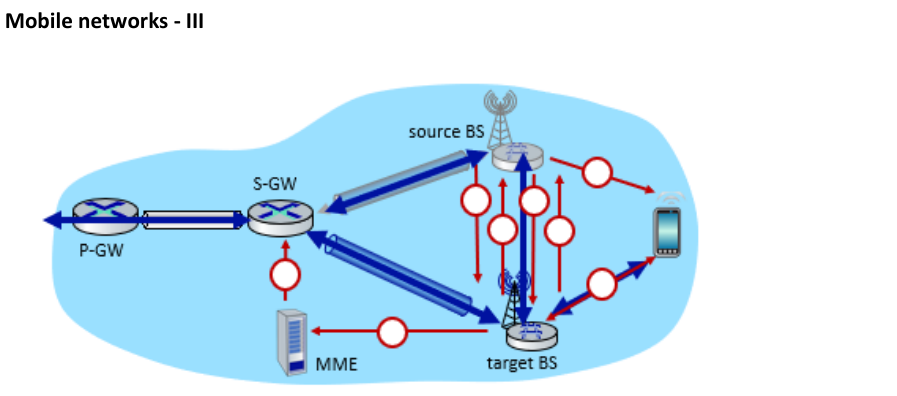
\includegraphics{images/questions/Schermata del 2023-11-02 10-47-37.png}
   % \caption{}
   \label{fig:dom2.6}
\end{figure}

L'immagine mostra l'handover di una connessione telefonica tra due base station appartenenti alla stessa rete telefonica in una rete 4G. L'handover è il processo di trasferimento di una chiamata o di una sessione dati in corso tra una base station e un'altra mantenendo la continuità di comunicazione. Questo processo è necessario quando un device si muove da una cella ad un'altra e il segnale della cella a cui era attaccato diventa troppo debole per mantenere la connessione.

In figura possiamo osservare la presenza di 7 step necessari per portare a compimento l'handover:

\begin{enumerate}
\item La BS corrente sceglie di selezionare un handover (per un deterioramento del segnale tra cellulare e BS o per overloading): seleziona una BS target e gli invia un \textbf{Handover Request message};
\item La BS target pre-alloca dei radio time slot, risponde con un \textbf{Handover Request ACK} con informazioni per il dispositivo mobile;
\item La BS sorgente informa il cellulare della nuova BS che ora può essere utilizzata per l'invio dei dati e così l'handover risulta completo dal punto di vista del al dispositivo mobile;
\item La BS sorgente allora termina l'invio di datagram al cellulare e invece inoltra alla nuova BS (che a sua volta inoltra al dispositivo mobile).
\item La target BS informa il MME (Mobile Management Entity) che è lei la nuova BS per il dispositivo, così il MME istruisce il S-GW per cambiare il tunnel endpoint per essere sulla nuova BS target.
\item La target BS invia un ACK di conferma del completamento dell'handover alla BS sorgente;
\item I dati inviati dal dispositivo mobile adesso passano attraverso la nuova BS e attraversano il tunnel creatosi con il S-GW.
\end{enumerate}

\section{SDN generalized forwarding}

\begin{figure}[htbp]
   \centering
   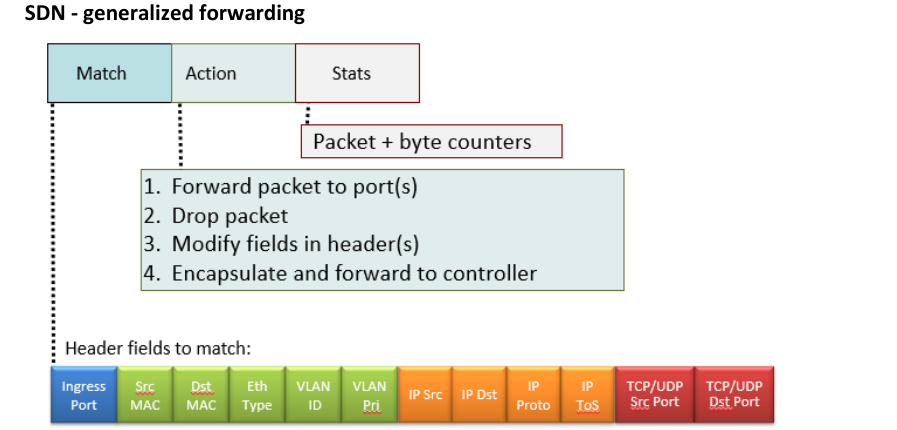
\includegraphics{images/questions/Schermata del 2023-11-02 11-34-36.png}
   % \caption{}
   \label{fig:dom2.7}
\end{figure}

Il generalized forwarding (approccio seguito da OpenFlow) è uno dei servizi implementati dal data plane SDN (Software-Defined Networking\footnote{SDN: approccio dove un controller remoto calcola e manda le forwarding tables ad ogni router}) e consiste nel fornire ad ogni router una forwarding table (o flow table) che usa l'astrazione ``match plus action\footnote{fare matching con i bits in arrivo, e di conseguenza effettuare quale azione inffettuare}". Il generalized forwarding utilizza diversi campi dell'header per determinare quale azione effettuare: le azioni possibili su un dato pacchetto/flusso sono \texttt{drop}, \texttt{forward}, \texttt{modify} e \texttt{send} (al controller).\\
La figura sopra rappresenta tutte le informazioni che possono essere usate su i diversi campi dell'header (link: verdi; network: arancioni; transport: rosse) per impostare le matching rules all'interno di una flow table.

L'astrazione ``match plus action" permette di unificare più tipi di device in base al loro comportamento:

\begin{itemize}
\item Router: il \texttt{match} è il prefisso IP più lungo, l'\texttt{action} è inoltrare verso un %(inoltro a tutti)
link
\item Switch: il \texttt{match} è i MAC address di destinazione, l'\texttt{action} è l'inoltro o il flood (inoltro a tutti) del pacchetto;
\item Firewall: il \texttt{match} è l'indirizzo IP e il numero di porta TCP/UDP, l'\texttt{action} permettere o negare il pacchetto;
\item NAT: il \texttt{match} è l'indirizzo IP e la porta, l'\texttt{action} di sostituire un indirizzo IP privato con un indirizzo IP pubblico
\end{itemize}

\section{SDN example}

\begin{figure}[htbp]
   \centering
   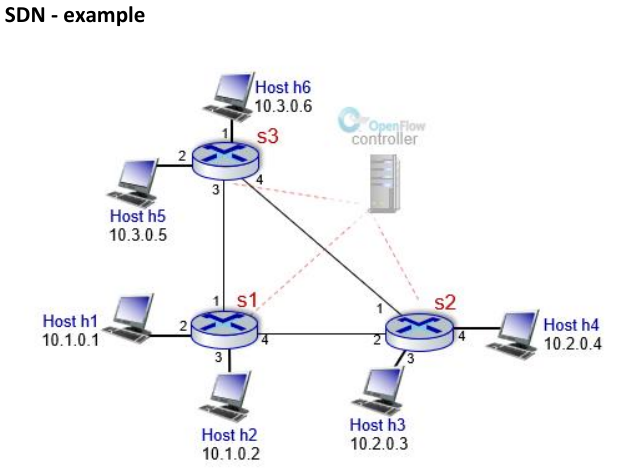
\includegraphics{images/questions/Schermata del 2023-11-02 11-52-53.png}
   % \caption{}
   \label{fig:dom2.8}
\end{figure}

Un semplice esempio di  rete SDN composta da 3 switch e 6 host in totale, l'SDN controller (nello specifico OpenFlow controller) programmerà gli switch in modo tale da inserire in ognuno di essi una flow table con tutte le regole di forwarding per la gestione del traffico di rete.

La cruciale differenza rispetto alle reti con switch tradizionali è il disaccopiamento fra control e data plane\footnote{Rispettivamente decidere dove il traffico deve essere indirizzato e indirizzarlo verso la giusta destinazione}, che invece di coesistere nei singoli device, sono separati permettendo una gestione centralizzata, opposta alla programmazione dei singoli switch. 

\note{Nel caso si volessero scrivere delle regole per far passare per \texttt{s1} i datagrammi provenienti dagli host \texttt{h5} e \texttt{h6} e destinati agli host \texttt{h3} e \texttt{h4}, le regole necessarie sarebbero:
\begin{itemize}
    \item \texttt{s3}: 
    \begin{itemize}
        \item \texttt{match}: IP Src = 10.3.*.*, IP Dest\footnote{Superfluo in questa specifica topologia, ma comunque opportuno metterlo} = 10.2.*.*;\texttt{action}: forward(3);
    \end{itemize}
    \item \texttt{s1}:
    \begin{itemize}
        \item \texttt{match}: ingress port = 1, IP Src = 10.3.*.*, IP Dest = 10.2.*.*; \texttt{action}: forward(4); 
    \end{itemize}
    \item \texttt{s2}: 
    \begin{itemize}
        \item \texttt{match}: ingress port = 2, IP Dest = 10.2.0.3; \texttt{action}: forward(3);
        \item \texttt{match}: ingress port = 2, IP Dest = 10.2.0.4; \texttt{action}: forward(4);
    \end{itemize}
\end{itemize}}

{\ns
Alcuni dei comandi chiave di OpenFlow ---discussi anche nella lezione di lab sul network slicing--- sono:
\begin{itemize}
    \item \texttt{features} richiede features allo switch
    \item \texttt{flowmod} aggiunge/elimina/modifica entries nelle table openflow 
    \item \texttt{packet-in} invia un pacchetto da switch a controller per farglielo gestire
    \item \texttt{packet-out} specifica la porta di output di uno switch per un pacchetto, eventualmente ricevuto con \texttt{packet-in}
\end{itemize}

Gli ultimi due comandi sono utilizzati ---ad esempio--- dal protocollo \texttt{LLDP}:
\begin{enumerate}
    \item Il controller genera un pacchetto LLDP per ogni porta attiva di ogni switch e lo invia con \texttt{packet-out}.
    \item Uno switch che riceve tale pacchetto dal controller lo inoltra agli switch adiacenti
    \item Uno switch che riceve tale pacchetto da un altro switch, lo incapsula in pacchetto LLDP e lo invia al controller con \texttt{packet-in}, aggiungendo \texttt{switchID}, \texttt{portID} e altri metadata.
    \item Il controller può ricostruire i link esistenti fra gli switch
\end{enumerate}
}

\section{SDN architecture}

\begin{figure}[htbp]
   \centering
   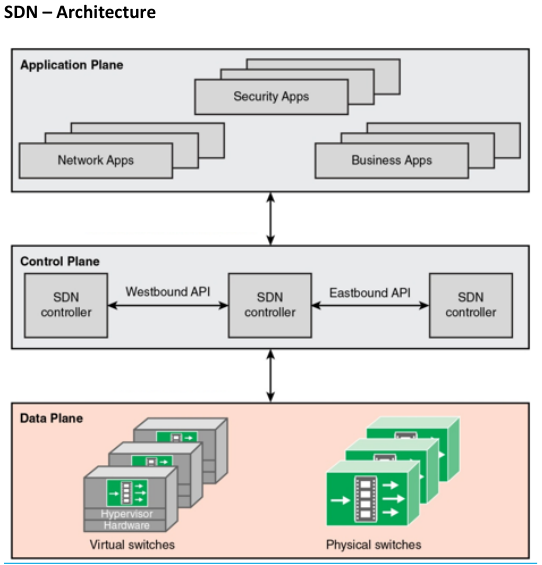
\includegraphics{images/questions/Schermata del 2023-11-02 15-17-26.png}
   % \caption{}
   \label{fig:dom2.9}
\end{figure}

L'immagine mostra l'architettura del SDN, partendo dal data plane, dove avviene il forwarding dei frame, passando per il control plane, dove avvengono le decisioni su dove indirizzare il traffico, fino ad arrivare all'application plane, che astrae dal control plane permettendo una gestione più intuitiva ---tipicamente con un approccio dichiarativo--- della rete.

L'architettura del data plane (quella evidenziata in figura) è composta principalmente da switch fisici e switch virtuali: ogni switch deve implementare un modello, o astrazione, di forwarding dei pacchetti basato sulle istruzioni fornite dai SDN controllers.\\
Il controller dialoga con gli switch del data plane attraverso un protocollo standardizzato denominato \textit{OpenFlow}. Questo protocollo consente al controller, attraverso comandi inviati su livello 2, di programmare gli switch affinché eseguano determinate azioni: in particolare abbiamo discusso del pattern \texttt{match + action}, ma non ci si limita a quello.

{\ns Alcune key features del data plane sono:
\begin{itemize}
    \item \textbf{Packet forwarding}: sono responsabili dell'inoltro pacchetti in base alle regole fornite dal controller.
    \item \textbf{Traffic shaping}: possono implementare politiche di traffic shaping per gestire il flow del network (e.g. dare priorità ad un certo tipo di traffico, come quelli voce o video, in modo che traffico prioritario sia inviato senza delay)
    \item \textbf{Security}: può implementare politiche di security shaping per prevenire accessi non autorizzati al network (e.g. filtrare pacchetti in arrivo da indirizzi notoriamente pericolosi)
    \item \textbf{QoS} (Quality of Service): può implementare politiche di QoS per assicurarsi che un certo tipo di traffico arrivi con un determinato grado di qualità.
    \item \textbf{Load balancing}: può implementare politiche di distribuzione del traffico per evitare congestioni e assicurarsi che il traffico sia efficientemente distribuito.
\end{itemize}}

Il SDN è definito su una serie di API che permettono l'interfacciamento con i vari livelli: dal control plane al data plane si parla di southbound API (e.g. OpenFlow), e permettono al control plane di ottenere informazioni sul traffico, e di conseguenza specificare le politiche di forwarding agli switches presenti nel data plane.
I controller espongono northbound API, permettendo a sviluppatori e a network managers di ``applicare" applicazioni network personalizzate.

\section{OpenFlow switch}

\begin{figure}[htbp]
   \centering
   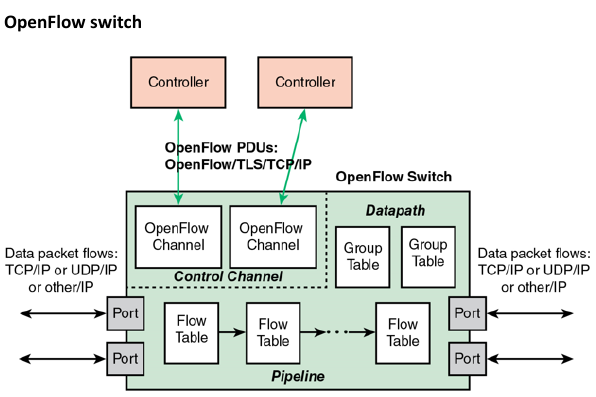
\includegraphics{images/questions/Schermata del 2023-11-02 15-30-18.png}
   % \caption{}
   \label{fig:dom2.10}
\end{figure}

Gli OpenFlow switch sono dispositivi di rete (fisici o virtuali) programmabili da OpenFlow controller, utilizzando comandi OpenFlow. Essi utilizzano una serie di flow table per gestire il traffico di rete, e sono formati dai seguenti componenti:

\begin{itemize}
\item Una serie di flow table organizzate in \textbf{pipeline}.
\item Una serie di \textbf{group table} all'interno del datapath, che permettono di specificare un comportamento più complesso che si riferisce a gruppi di flusso (stabilendo regole basate sugli attributi dei flussi).
\item Gli OpenFlow Channels supportano la comunicazione con i controller nel control plane. Tipicamente gli switch sono collegati a più controllers, dato che è possibile avere una serie di controlli distribuiti. La configurazione più semplice è quella dello master-slave, con un solo controller che comunica con lo switch, altre più complesse fanno uso di più controller con ridondanza "active-passive".
\item Ports: questi switch hanno diversi tipi di porte, tra cui porte fisiche, porte logiche (versioni virtualizzate di quelle fisiche)  e porte riservate.
\end{itemize}

Le flow table sono disposte a pipeline all'interno dello switch. Quando un pacchetto entra nella pipeline, inizierà a scorrere la prima tabelle fino a quando non troverà un match in una delle tabelle. Se ci sono più match in una table, verrà selezionato quello con priorità più alta. Se l'unico match è quello di \textit{table-miss entry\footnote{match di default che specifica il comportamento dello switch in caso un pacchetto non effettui un match con nessun'altra regola}}, allora una delle tre azioni è possibile:

\begin{itemize}
    \item passare il pacchetto alla successiva flow table (se presente).
    \item delega al controller: il pacchetto viene delegato al controller, che in base alle politiche a lui assegnate deciderà se creare un nuovo flow per quel pacchetto, oppure dropparlo.
    \item droppare il pacchetto.
\end{itemize}

\section{Interazione control plane/data plane}

\begin{figure}[htbp]
   \centering
   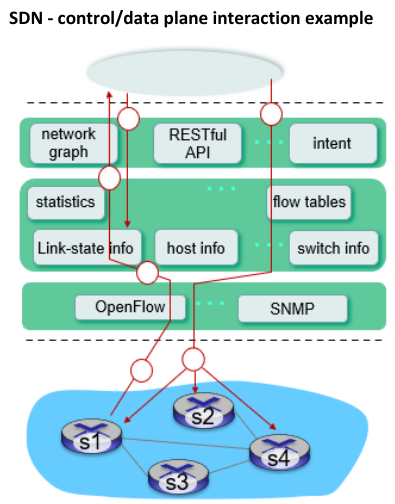
\includegraphics[width=0.3\textwidth]{images/questions/Schermata del 2023-11-02 17-04-24.png}
   % \caption{}
   \label{fig:dom2.11}
\end{figure}

Il controller è suddiviso in:
\begin{itemize}
    \item  API di astrazione per interfacciarsi con le applicazioni di network control.
    \item Database distribuito su stato di link, switch, servizi, ecc\dots
    \item Componenti comunicazione con gli switch
\end{itemize}

L'immagine mostra un esempio di interazione tra il control plane e il data plane nel caso in cui uno switch rilevi un errore in uno dei suoi collegamenti (il link da \texttt{s1} a \texttt{s2}). Tale interazione è composta da 6 step totali:

\begin{enumerate}
\item Lo switch S1 ha un errore di collegamento (poiché ha perso il link a S2), quindi invia un OpenFlow \texttt{port-status} message per notificare il controller;
\item SDN Controller riceve il messaggio e aggiorna le informazioni di stato di quel link;
\item Ipotizzando che l'applicazione che implementa l'algoritmo di Dijkstra per il routing sia eseguita fuori dal controller, sarà compito del controller avvisare tale applicazione del nuovo stato della topologia di rete.
\item L'applicazione accede alle informazioni del grafo di rete, alle informazioni dello stato dei link e calcola nuove rotte;
\item L'applicazione di link state routing interagisce con il componente che produce le flow-table nel controllore SDN, che calcolerà le nuove flow table;
\item Il controller infine usa OpenFlow per installare le nuove flow-table negli switch che devono essere aggiornati inoltrando un \texttt{flow-mod} message agli switch
\end{enumerate}

\section{NFV forwarding graph}

\begin{figure}[htbp]
   \centering
   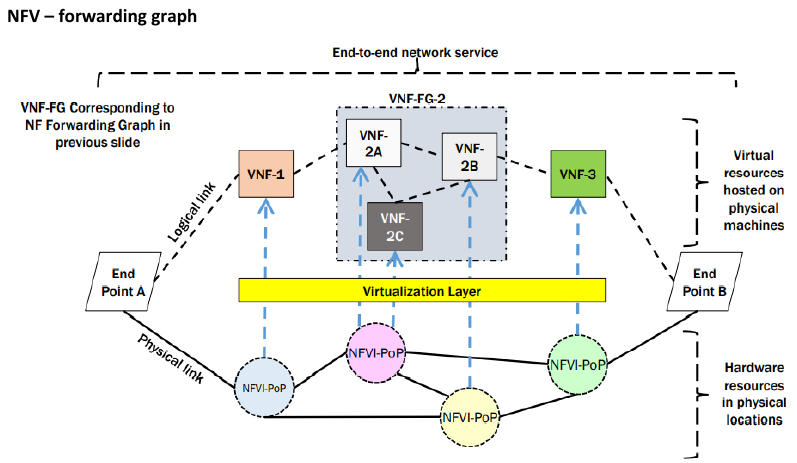
\includegraphics{images/questions/Schermata del 2023-11-02 17-23-22.png}
   % \caption{}
   \label{fig:dom2.12}
\end{figure}

Il crescente utilizzo di internet e di servizi che richiedono connessioni brevi ad alta velocità hanno portato alla necessità di acquisto di hardware specializzato per ognuna delle funzioni richieste, portanto ad una distribuzione ad alta densità di infrastrutture network. Gli operatori di rete stanno progressivamente passando da soluzioni basate solo su hardware a soluzioni basate anche su software. La NFV (Network Function Virtualization) affronta questi problemi sfruttando le tecnologie di virtualizzazione: permette di \textbf{disaccoppiare} l'hardware dal software, consentendo di migrare ed eseguire funzioni di rete dove necessario. 

Un network service può essere scomposto in un insieme di \textit{Virtual Network Functions} (VNF) (e.g. Firewalls, IDS, load balancers, ...)pu, quindi può essere anche visto come un forwarding graph di network function e endpoint. I link logici che interconnettono ogni network function possono essere gestiti tramite controllori SDN e devono essere supportati da path fisici attraverso l'infrastruttura di rete sottostante.

\note{Ogni network service può essere implementato da un singolo operatore o da una rete di più operatori.}

Un network service può essere composto da una o più VNF che sono deployate attraverso l'uso di VM (Virtual Machine) o container (in questo caso si parlerebbe di CNF (Containerized Network Function)), i quali comunque devono essere ospitati da una macchina fisica, detta \textit{Point of Presence} (\textbf{PoP}).
Il problema del \textbf{collocamento} delle VNF non è banale e deve tenere conto di QoS (latency e min bandwidth), performance, bandwidth, risorse PoP, massimizzando una \textit{utility function}.
L'ottimalità può essere definita in base a vari fattori, come latenza complessiva, costo deployment, bandwidth utilizzata\dots
Non c'è una soluzione standard al problema, i requisiti possono essere variabili e gli approcci per risolverlo altrettanto diversificati, e.g. algoritmi genetici, ML, programmazione lineare.

Un esempio applicabile all'immagine potrebbe essere: \texttt{VFN-1} servizio di cache posizionato vicino all'end point (quindi sull'edge della rete). È possibile che una VNF sia composta da diverse VNF, come accade in figura per \texttt{VFN-FG-2}.
È possibile che le performance di un servizio possano benificiare da una corrispondenza fra link logici e fisici: un servizio di cache o firewall istanziato sul nodo fisico più lontano  dall'endpoint ingress può significare multipli hop per dati che dovrebbero invece avere un rapido accesso.

Grazie alla virtualizzazione è possibile migrare e istanziare dinamicamente VNF e allocare risorse a seconda delle necessità, ed eventualmente automatizzare il tutto grazie ad un orchestrator. 


\section{NFV MANO}

\begin{figure}[htbp]
   \centering
   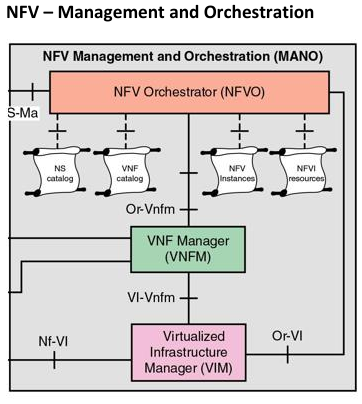
\includegraphics{images/questions/Schermata del 2023-11-03 12-20-29.png}
   % \caption{}
   \label{fig:dom2.13}
\end{figure}

La figura mostra la struttura interna di un NFV MANO formato da diverse componenti, le principali delle quali sono: NFVO (o NFV Orchestrator), VNFM (o VNF Manager) e VIM (o Virtual Infrastructure Manager). Questi componenti forniscono le funzionalità richieste per istanzare i VNFs, fornendo le configurazioni dei VNFs e le configurazioni all'infrastuttura in cui i VNFs verranno eseguiti. 

Utilizzando un approccio top-bottom troviamo:
\begin{itemize}
    \item il NFV (NFV Orchestrator), responsabile della creazione, dell'installazione, della configurazione, e del lifecycle dei network services, composti a loro volta da pacchetti di VNF. Questo componente fa affidamento a delle repositories per ottenere informazioni sui servizi:
    \begin{itemize}
        \item il \textit{NS Catalog}, è una repository che contiene una lista di network services utilizzabili (con relativi deployment templates per NS in termini di VNFs)
        \item il \textit{VNF Catalog}, una repository contenente tutti i VNFD (descrittori che descrivono le funzioni da un punto di vista delle risorse necessarie per poter istanziare tale funzione)
        \item \textit{NFVI} (Network Function Virtualization Infrastructure) \textit{resources}, repository con lista di risorse necessarie per costruire e mantenere l’infrastruttura NFV e i servizi attivi.
        \item \textit{NFV instances}, repository con lista contenente dettagli relativi al deployment dei network services e corrispondenti VNF.
    \end{itemize}

    \note{L'orchestrator si occupa anche di comunicare con componenti hardware di rete tradizionali}
    
    Il collegamento \texttt{Se-Ma} permette di far arrivare le richieste di network service \textred{da un manifesto contenente i dettagli richiesti di rete?}.
    
    \item il VNFM (VNF Manager), responsabile della gestione del ciclo di vita di ogni singola VNF. Si occupa di istanziazione, aggiornamento, query, di aumentare o diminuire il numero di istanze (scale up/down) e infine di terminare una VNFI (VNF Instance). È anche il responsabile della raccolta di metriche delle VNFs, e di informazioni legate ad eventuali fault/errori.
    
    \item il VIM (Virtualized Infrastructure Manager), responsabile del controllo e della gestione dell'interazione di una VNF con le risorse di computing, storage e rete dell'infrastruttura fisica sotto il suo controllo (e.g. per un network service serve un set di VM con determinate caratteristiche). Una singola istanza di VIM è in grado di gestire un intero dominio d'infrastruttura\footnote{set di risorse fisiche e virtuali gestite da un operatore di rete in una specifica area} sotto il controllo di un operatore. Per amministrare l'intera rete, potrebbero essere necessarie più istanze di VIM in un singolo MANO.
\end{itemize}

\section{Esempio di network slicing}

Il network slicing è una tecnica utilizzata nelle reti SDN (Software Defined Network) per isolare le risorse di rete e soddisfare diverse esigenze su un'infrastruttura fisica condivisa. 

Questa immagine illustra l'implementazione del network slicing in un SDN per consentire l'isolamento delle risorse di rete. L'obiettivo di questo esempio è mostrare che diverse necessità possono essere soddisfatte utilizzando il network slicing su un'infrastruttura fisica condivisa. L'architettura impiega una topologia multi-hop: la rete comprende quattro host (h1, h2, h3, h4) e quattro switch (s1, s2, s3, s4). La rete deve essere isolata in due slice per due servizi:
\begin{itemize}
    \item Slice del traffico video (upper slice): Il traffico video (porta UDP 9999) può utilizzare un massimo di 10 Mbps di larghezza di banda. Il diritto del traffico video di utilizzare questa larghezza di banda non è influenzato dagli altri tipi di traffico.
    \item Slice per altri tipi di traffico (lower slice): Tutti i traffici, che non siano di tipo UDP porta 9999, possono utilizzare qualsiasi percorso della rete, ma non devono influenzare il traffico video.
\end{itemize}

\note{Tutti gli switch sono collegati (anche se non mostrato in figura) ad un controller.}

\begin{figure}[htbp]
   \centering
   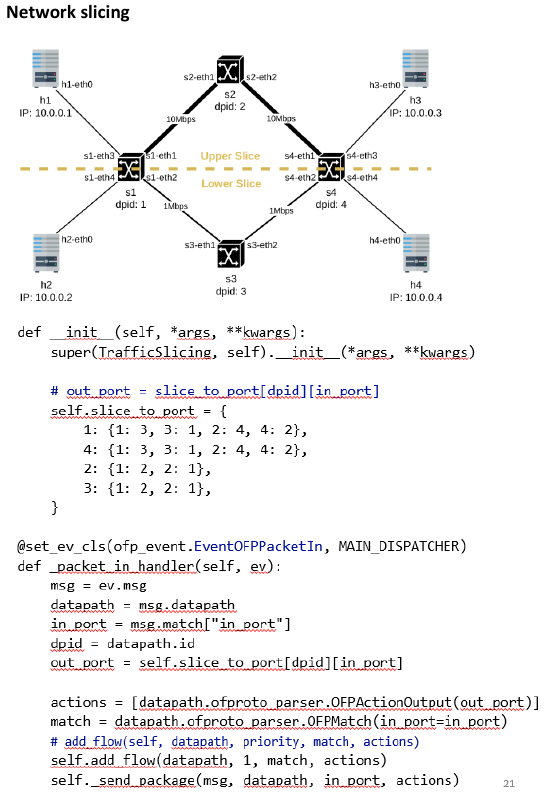
\includegraphics[width=0.49\columnwidth]{images/questions/Schermata del 2023-11-03 14-33-14.png}
   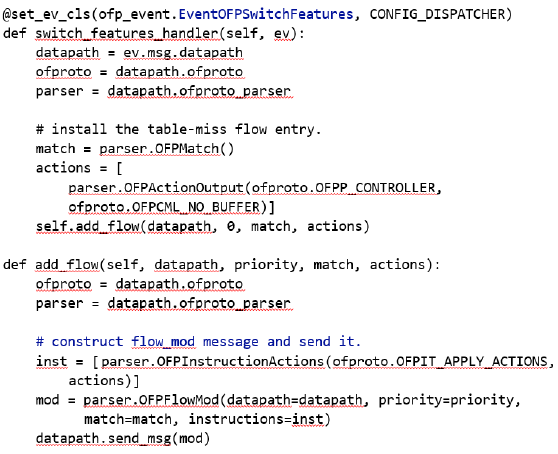
\includegraphics[width=0.49\columnwidth]{images/questions/Schermata del 2023-11-03 14-33-37.png}
   % \caption{}
   \label{fig:dom2.14.1}
\end{figure}

Il codice mostrato definisce il comportamento del \textit{controller} in alcune situazioni.

Nel primo snippet, c'è una entry di un dizionario per ciascuno switch, e per ciascuna di queste il mapping delle porte che definisce deve essere inoltrato il traffico.
In sostanza qui si definiscono le informazioni necessarie per generare le regole di flusso, che dovranno poi essere applicate agli switch.

\note{La topologia viene implementata nel file network.py, e definisce hosts, switch, e collegamenti fisici.}

Un'applicazione Ryu può registrare l'ascolto di specifici eventi, con handler da lanciare una volta rilevato l'evento. Il primo evento descritto nell'immagine è quello di packet in (\lstinline{EventOfPacketIn}), quindi in \lstinline{_packet_in_handler} viene definito il comportamento per un pacchetto in arrivo.
Il controller riceve dagli switch un \textit{packet in} message, permettendogli di sapere ID switch e porta ingress del pacchetto, e dunque di comunicare allo switch il flow e le azioni da eseguire utilizzando la funzione \lstinline{add_flow}, in base allo slicing del primo snippet.
\lstinline{_send_package} invia allo switch un \textit{packet out} message per gestire lo specifico pacchetto che lo switch non aveva saputo gestire, e per cui quindi aveva invia un \textit{packet in} message al controller.

\note{In questo modo, la prima volta che arriva un pacchetto, lo switch lo invia al controller il quale determina su quale porta dello switch debba essere inoltrato (in base alla topologia definita) e glielo comunica. Poi lo switch manderà autonomamente pacchetti con tale ingress port sulla porta output indicata.}

\lstinline{switch_features_handler} serve per gestire l'evento di ricezione di un messaggio di \textit{feature reply}  (\lstinline{EventOfPSwitchFeatures}), mandato in risposta dagli switch al periodico \textit{feature request} dei controller.
Lo snippet, alla ricezione di tale messaggio, installa nello switch una entry con un \lstinline{flow_mod} message per indicare allow switch di propagare al controller la gestione dei pacchetti qualora non trovasse un match nelle sue table. \\
In sostanza \lstinline{match} = \textit{nessuna entry disponibile} + \lstinline{action} = \textit{inoltra a controller}.

\lstinline{add_flow} costruisce un messaggio \lstinline{flow_mod} in base ai parametri e poi lo invia a \lstinline{datapath}, che è un oggetto che incapsula l'ID e l'address dello switch destinatario.

\section{Serie di Fourier}

\begin{figure}[htbp]
   \centering
   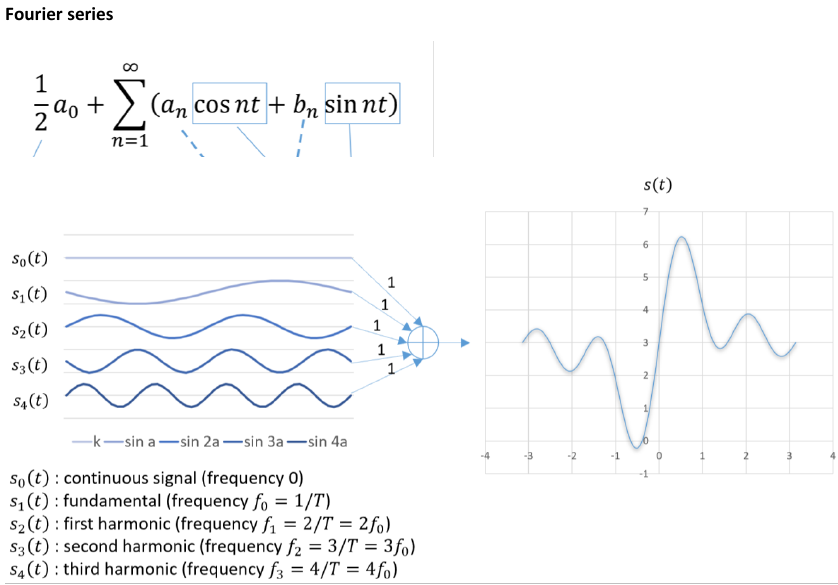
\includegraphics[width=0.55\columnwidth]{images/questions/Schermata del 2023-11-03 14-44-22.png}
   % \caption{}
   \label{fig:dom2.15}
\end{figure}

L'immagine in figura mostra la definizione della serie di Fourier, utilizzata per la decomposizione di un segnale continuo e periodico (in $[-\pi,\pi]$) nei suoi armonici (che sono generalmente funzioni trigonometriche che oscillano a diverse frequenze). Possiamo vedere come $s(t)$ a destra sia formato dalla composizione delle 4 armoniche fondamentali e da una componente costante $s_0(t)$. Sopra abbiamo invece l'equazione che definisce le serie di Fourier per $s(t)$ definita da $\mathbb{R} \xrightarrow{} \mathbb{R}$ nell'intervallo $[ -\pi, \pi ]$: è utilizzata per decomporre il segnale in una somma di funzioni continue infinite (periodiche e che oscillano a diverse frequenze), dove:

\begin{align}
a_0 &= \frac{1}{\pi} \int_{-\pi}^{\pi} s(t)dt\\
a_n &= \frac{1}{\pi} \int_{-\pi}^{\pi} s(t)cos(nt)dt\\
b_n &= \frac{1}{\pi} \int_{-\pi}^{\pi} s(t)sin(nt)dt\\
\end{align}

$a_0$ è la componente costante, $sin(nt)$ e $cos(nt)$ sono gli armonici, mentre $a_n$ e $b_n$ sono le rispettive ampiezze degli armonici.
Non sono conosciute le condizioni \textit{necessarie} per cui $s(t)$ possa essere sviluppata in una serie di Fourier, ma esistono due condizioni \textit{sufficienti} (\textit{Dirichlet}):

\begin{itemize}
\item $s(t)$ sia periodica
\item $s(t)$ sia continua a tratti
\item[$\Rightarrow$] ed è possibile affermare che in questo modo la serie di Fourier di $s(t)$ esiste e converge in $\mathbb{R}$
\end{itemize}

La serie di Fourier può anche essere scritta con base esponenziale, sfruttando l'esponenziale di eulero (periodo $T = \nicefrac{1}{F}$):
\[s(t) = \sum_{n=-\infty}^{+\infty}S_n e^{j 2 \pi n F t} = \sum_{-\infty}^{+\infty}S_n(cos(\pi n F t) + jsin(\pi n F t))\text{, con }S_n = \frac{1}{T}\int_{0}^{T}s(t) e^{- j 2 \pi n f t}dt\]

\note{$S_n$ rappresenta il contributo (\textit{ampiezza}) di ciascuna funzione $e^{- j 2 \pi n f t}$ al nostro segnale di partenza $s(t)$}

Qualora un segnale fosse non periodico non se ne può ottenere la serie di Fourier, in quanto per un tale segnale avremmo che il periodo tendente ad infinito $T\rightarrow\infty$ e di conseguenza una frequenza fondamentale $F = \nicefrac{1}{T} \rightarrow 0$, portando gli armonici (multipli di $F$) ad essere infinitamente vicini gli uni agli altri.
In tal caso si può applicare la \textit{\textbf{Trasformata di Fourier Continua}}, che restituisce lo \textit{Spettro} $S(f)$ del segnale, indicante come il segnale è distribuito nel campo delle frequenze.
\[S(f) = \int_{-\infty}^{+\infty}s(t) e^{- j 2 \pi n f t}dt\text{, con }s(t)\text{ segnale non periodico: } s(t) = \int_{-\infty}^{+\infty}S(f) e^{ j 2 \pi n f t}dt\]

\section{DFT (Discrete Fourier Trasform)}

\begin{figure}[htbp]
   \centering
   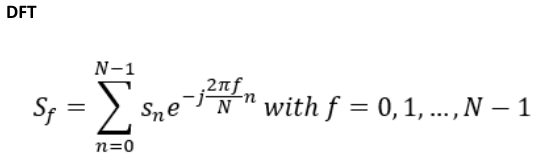
\includegraphics{images/questions/Schermata del 2023-11-04 16-30-36.png}
   % \caption{}
   \label{fig:dom2.16}
\end{figure}

Abbiamo visto come la serie di Fourier permetta di scrivere un segnale continuo e periodico (in un intervallo) come la somma di segnali, o meglio, \textit{armonici}.
La trasformata di Fourier ci permette di ottenere la serie ordinata di coefficienti di ampiezza degli armonici $S_n$, detta \textit{Spettro} del segnale.
Il valore assoluto di $|S_f|$ rappresenta l'ampiezza dell'armonico di frequenza $f=1/N$, con $f$ frequenza fondamentale.

\note{Ciascun armonico è la somma di $sin$ e $cos$, ciascuno moltiplicato per un coefficiente indicante l'\textit{ampiezza} (in modo informale il ``peso'' dell'armonico).
La serie di Fourier può anche essere scritta con base esponenziale, sfruttando l'esponenziale di eulero (periodo $T = \nicefrac{1}{F}$:
\[s(t) = \sum_{n=-\infty}^{+\infty}S_n e^{j 2 \pi n F t} = \sum_{-\infty}^{+\infty}S_n(cos(\pi n F t) + jsin(\pi n F t))\]
\[ s(t) = \sum_{n=-\infty}^{+\infty}S_n e^{ j 2 \pi n F t} \quad S_n = \frac{1}{T}\int_{0}^{T}s(t) e^{- j 2 \pi n F t}dt\]
In effetti $e^{j\Theta} = cos(\Theta) + jsin(\Theta)$}

La trasformata di Fourier di un segnale continuo ma \textit{non periodico} sfrutta l'esponenziale di Eulero, e prevede di integrare da $-\infty$ a $+\infty$; ciò avviene perché per rappresentare un segnale non periodico diciamo che abbia periodo $T\rightarrow\infty$, e che dunque gli armonici siano potenzialmente infiniti. Dunque il risultato fornisce non una serie di coefficienti, bensì lo \textit{spettro} $S(f)$ del segnale continuo $s(f)$:
\begin{equation}
\label{eq:FT_periodic}
S(f) = \int_{-\infty}^{+\infty}s(t) e^{- j 2 \pi f t}dt
\end{equation}
\note{Per segnali non periodici, la situazione si complica un po'.}

La funzione in figura rappresenta la definizione di una trasformata di Fourier discreta, da applicare a un discreto non continuo.
Tale segnale si ottiene tramite il \textit{sampling} di un segnale continuo, che fornisce una serie di osservazioni separate da un intervallo di tempo $T$.

Dato che tali osservazioni sono ``puntiformi'' nel grafico, si assume  che ogni sample abbia un \textit{``impulso''} (i.e. un rettangolo nel piano), dunque invece di calcolare un integrale come in \ref{eq:FT_periodic}, si scompone tale integrale in una sommatoria che arriva fino ad $N$, ovvero il numero di osservazioni.

\[ S(f) = \int_{-\infty}^{+\infty}s(t) e^{- j 2 \pi f t}dt = s(0) e^{- j 2 \pi f 0} + s(1) e^{- j 2 \pi f 1} + \ldots + s(N-1) e^{- j 2 \pi f (N-1)}\]
\[ \text{i.e. }S(f) = \sum_{0}^{N-1}s(t) e^{- j 2 \pi f n}, n \in \{0, 1, \ldots, N-1\}\]

Dato che i sample sono divisi da un tempo $T=\nicefrac{1}{N}$ sono periodici, prendiamo $f$ non in $\mathbb{R}$, bensì nell'insieme della frequenza fondamentale $\nicefrac{1}{N}$ e dei suoi multipli (armonici) $f = 0,\nicefrac{1}{N},\nicefrac{2}{N},\dots,\nicefrac{N-1}{N}$.\\
Per comodità di notazione nella formula riportata, $f=0,1,\dots,N-1$ e nell'esponente si divide per $N$.

Quindi considerando tutte queste assunzioni, la formula nell'immagine mostra come è possibilie calcolare la trasformata di Fourier discreta, a partire da un numero finito di sample di un segnale. La formula inversa per ottenere i valori dei sample è la seguente:

\[ s_n = \frac{1}{N} \sum_{0}^{N-1} S_f e^{j 2 \pi f \frac{n}{N}}\]

% \newpage
\section{Sampling and Aliasing}
\begin{figure}[htbp]
    \centering
    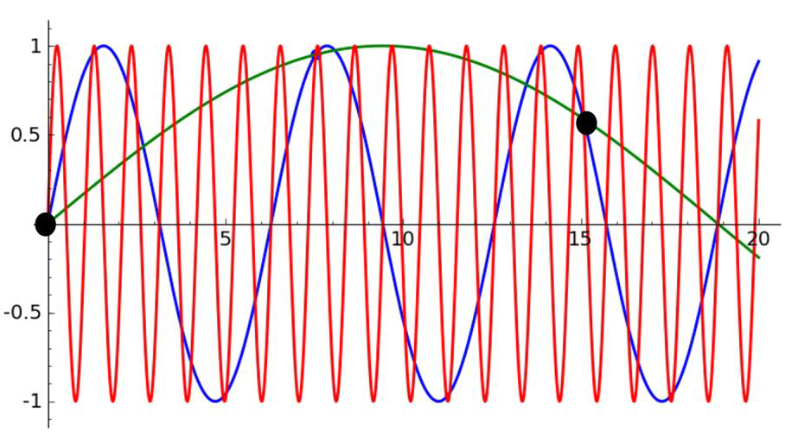
\includegraphics{images/questions/sampling_aliasing.png}
    % \caption{Caption}
    \label{fig:sampling_aliasing}
\end{figure}

Ci sono due tipi di errori che rendono la trasformata di Fourier discreta diversa rispetto allo spettro del vero segnale sul quale sono stati effettuati i samples:
\begin{itemize}
    \item Aliasing: non utilizzare un rate di sampling appropriato per un segnale che varia molto frequentemente in un periodo potrebbe portare a difficoltà nel ricostruirlo e nell'analisi del comportamento della sua frequenza.
    Per esempio, dati dei sample, applicando la FT è possibile risalire a un segnale che abbia come spettro anche una sola frequenza che corrisponda al segnale campionato, quando invece questi potrebbe essere la somma di più armonici, oppure semplicemente ad un armonico della frequenza fondamentale ($s(t)$ e $3s(t)$ potrebbero apparire uguali da campionati).\\
    Nell'immagine le tre sinusoidi differiscono di \nicefrac{1}{6}, i.e. $f' = \nicefrac{f}{6}$, e matchano tutte i campioni neri, ma sono tre segnali diversi!
    %Questo effetto è noto come \textbf{aliasing}.
    \item Leakage: durante il sampling di un segnale periodico, può accadere che il primo e l'ultimo sample del periodo abbiano valori diversi (presumibilmente a causa di un'interruzione di sampling non avvenuta a fine periodo). Questo porta a discontinuità tra gli end-point dei sampling periodici, creando possibili false ricostruzioni. 
    \note{Per arginare il problema, una soluzione potrebbe essere quella di far tendere a 0 il primo e l'ultimo sample.}
\end{itemize}

Un segnale discreto $g(nT)$ si può ottenere con un sampling uniforme di un segnale continuo $s(t)$:
\[ g(nT) = s(nT) \]
Dove $T$ è il periodo di sampling mentre $F=\nicefrac{1}{T}$ la frequenza di sampling.

%Intuitivamente un segnale che cambia rapidamente dovrà essere campionato ad alta frequenza. Il Sampling Theorem ci dice che in condizioni ideali la frequenza minima di campionamento per poter poi ricostruire un segnale continuo è la \textit{frequenza di Nyquist}:

Sapendo che $f_M$ è il limite oltre il quale lo \textit{spettro} di $s(t)$ è nullo, il Sampling Theorem ci dice che $s(t)$ è rappresentata dai suoi campionamenti se:
\begin{enumerate}
    \item essi avvengono in intervalli regolari $t_n = nT_c$ (con $n \in \mathbb{Z}$)
    \item con un periodo di sampling di $T_c \leq \frac{1}{2f_M}$, o detto in altri termini, la frequenza minima di campionamento deve essere:
\end{enumerate}

\begin{equation}
    f_{c_{min}} = \frac{1}{T_{c_{max}}} = 2f_M \rightarrow \text{\textit{frequenza di Nyquist}}
\end{equation}
%Dove $f_M$ è il limite oltre il quale lo \textit{spettro} di $s(t)$ è nullo.
In altre parole, $f_{c_{min}}$ è il doppio della frequenza più alta in $s(t)$.
Soddisfatte queste condizioni, il segnale originale può essere ricostruito tramite interpolazione.

%Dati dei sample applicando la FT è possibile risalire a un segnale che abbia come spettro anche una sola frequenza che corrisponda al segnale campionato, quando invece questi potrebbe essere la somma di più armonici, oppure semplicemente ad un armonico della frequenza fondamentale ($s(t)$ e $3s(t)$ potrebbero apparire uguali da campionati).\\
%Nell'esempio le tre sinusoidi differiscono di \nicefrac{1}{6}, i.e. $f' = \nicefrac{f}{6}$, e matchano tutte i campioni neri, ma sono tre segnali diversi!
%Questo effetto è noto come \textbf{aliasing}.

Il motivo per cui Nyquist richiede che i segnali abbiano un tetto massimo di frequenza è che ciò permette di evitare di considerare frequenze più elevate che matchino i campioni osservati.
Il vero limite di Nyquist, più della frequenza di sampling richiesta, è proprio richiedere l'esistenza di tale tetto massimo sulla frequenza del segnale, difficile da riscontrare nel mondo fisico (nel mondo reale la situazione raramente è ``ideale''): nessun segnale è perfettamente limitato in banda. Anche se un segnale è limitato in frequenza, non è possibile campionarlo e ricostruirlo perfettamente a meno di non prendere un numero infinito di campioni.

\note{Il teorema stabilisce una frequenza minima di campionamento, ma non il numero di campioni necessari, il che implica che un numero finito di campioni non può garantire una ricostruzione perfetta.}

Un problema che potrebbe avvenire se il tetto massimo di frequenza non è selezionato correttamente è quello di ricostruzione non accurata. Questo perché la distanza tra il centro di una replica e il centro di un'altra è proprio la frequenza di campionamento, quindi più questa frequenza è alta, più le repliche del segnale periodico sono distanti una dall'altra. 

Detto ciò, il teorema fornisce comunque una buona base (periodo di sampling) per una ricostruzione che è sufficientemente accurata per le necessità applicative, considerando che comunque esistono segnali che sono quasi limitati in banda (e.g. voce). In caso è anche possibile applicare dei filtri (non esistono filtri ideali, ci sarà sempre un margine di errore) per eliminare delle frequenze sopra una certa soglia, in modo da soddisfare meglio i requisiti del teorema.

%\textred{Non ho capito il discorso delle repliche shiftate}

% \newpage
\section{Quantization}

\begin{figure}[htbp]
    \centering
    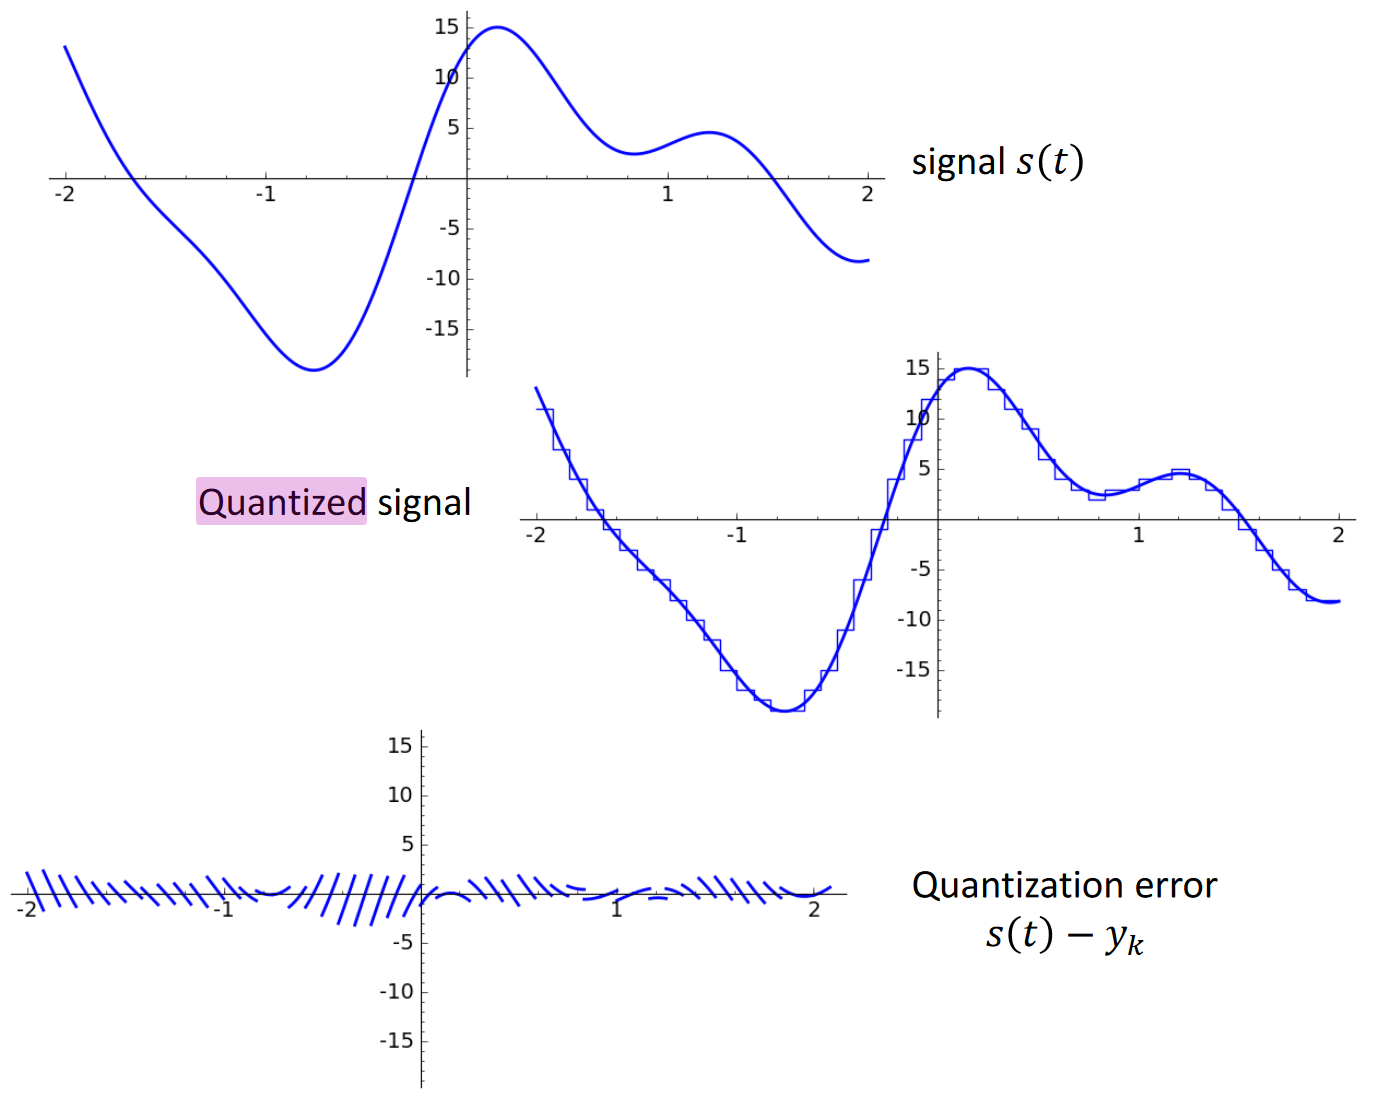
\includegraphics{images/questions/quantization.png}
    % \caption{Caption}
    \label{fig:quantization}
\end{figure}

Quantizzare con un ``quantizzatore scalare a $R$-bit''. significa approssimare il valore di un sample $x_k$ in un intero $y_k$ rappresentabile nel range $[0,2^R - 1]$ (e.g. Arduino usa 10 bits). Questo è necessario perché la rappresentazione dei sample in floating point (4 o 8 byte) potrebbe essere non possibili a causa di restrizioni hardware (caso comune in IoT). Più bit sono disponibili, più la risoluzione della quantizzazione è alta. Applicando una quantizzazione uniforme, la risoluzione di un segnale con valori tra $[0, M]$ è di $\frac{M}{R^2}$.

Chiaramente tale approssimazione porta un errore nella nella rappresentazione del sample ---e nell'eventuale ricostruzione del segnale---, che in casi estremi può sfociare nell'\textbf{overload} ($s(t) > 2^R - 1$) o nella mancata osservazione di \textbf{rumore granulare}, i.e. il segnale varia talmente poco in un intervallo $I_k$ che viene rappresentato con un unico $y_k$.